\chapter{Reorganization of Functional Network Architecture During Language and Reading Comprehension}

\section{Reading plugs into language systems}
Most current cognitive models suggest that language comprehension requires the construction of a mental representation includes textual information and associated background knowledge, connected by some conscious and some unconscious executive processes (Kendou et al., 2014). Thus, while there may be a core set of systems for manipulating and extracting meaning from language, it is quite possible that there are modality-specific influences on these systems 

Word recognition and oral language comprehension are strong predictors of reading comprehension skill (Gough/Tumner, 1989; Expanded simple view). Furthermore, many of the most dramatic changes associated with reading acquisition are linked to the reorganization of visual or phonological systems, areas not directly related to semantic or comprehension processes (Schlaggar, 2006; Dahaene 2015). Substantial evidence from two decades of neuroimaging suggests that inputs, from auditory or visual domains are fed up into higher-order association areas that sequence, encode articulatory plans, and extract semantic information (Price, 2012). These processes localize onto the similar areas regardless of language and writing system (Rueckl et al., 2016), and may even extend to inputs from somatosensory or non-linguistic domains (Xu et al., etc.). This supra-modal language core is largely left-lateralized and centers on the inferior frontal gyrus, anterior and posterior middle temporal gyrus and the angular gyrus. 

However, there is evidence that comprehending written and spoken language are not equivalent. There is a subset of students who, despite adequate word decoding skills and vocabulary skills, struggle with reading comprehension (Nation \& Snowling…, Spencer, Quinn \& Wagner). More on SRCD. From a neurobiological perspective, expected differences in primary visual (for reading) and primary auditory (for listening) represent the different input systems, with ventral occipito-temporal systems also activating (e.g., Jobard et al., 2007). However, differences in core language systems are also observed: additional activation in left posterior temporal and parietal areas in reading modality (Constable et al., 2015), as well increased bi-laterality (Berl et al., 2010), especially in children. 

These modality-specific influences – sometimes termed “fingerprints” – on behavior and brain activity may arise from a few different sources: subject, linguistic and innate differences. 

\subsection{Subject-Dependent Differences}
As disussed above, reading is a learned skill with may component processes. It requires thousands of hours of experience to master and entails a reorganization of cortical resources. Environmental and biological factors thus exert a greater influence on an individual’s reading proficiency than they might on more intrinsic processes such as speech comprehension. This is particularly dramatic in individuals with dyslexia, who have persistent difficulty with reading. Children with dyslexia exhibit less activation in reading-related areas compared to typically developing children (Pugh et al., 2000), but greater activation in right hemisphere homologues, suggesting that lateralization and activation of the reading circuit are associated with better reading. Development period also has an effect, with children exhibiting less activation in frontal areas but more in posterior areas, possibly reflecting a shift in “resource load” from uni-modal to supramodal areas (Berl et al., 2010). This shift may not be necessary in listening, or occur much earlier. Thus, with increasing expertise and development, there may be a “shift” from relying on fusiform processing areas. towards using multi-modal areas more like speech (Monzalvo et al.). 

\subsection{Language-Dependent Differences}
People speak differently than they write. Reading often relies on more complicated syntax, and even for skilled readers, longer words and sentences can strain executive systems more than they might if being spoken to. Although these properties are often controlled for in scientific studies, they represent a major difference between “natural” reading and listening. Because of these differences, reading may place a greater load on executive function skills. Executive functions such as working memory and planning and organizing may be particularly important for reading (Cain/Oakhill, Cutting).  

\subsection{Modality-bound differences}

Speech contains overt clues about the speaker, such as tone and prosody, and these can convey additional non-linguistic meaning for the listener. Reading, on the other hand, might be considered a more purely linguistic act, especially with computer-printed text. Reading may thus allow more room for self-generated situation models and more independent direction of thought. Furthermore, modality-specific aspects of the stimulus may influence the overall comprehension process; reading requires a level of spatial awareness -where one is at on a page, what happened in preceding paragraphs – and allows for the re-treading of information. Listening, meanwhile, requires the extraction of input from competing noises and sometimes the tracking of changing volume. 

Our central argument is that, just because language possesses supra-modal processing areas does not indicate that language is entirely supra-modal. Just as there is considerable evidence for supra-modal processing, there is also evidence for modality fingerprints on language comprehension. These influences may arise from the intrinsic organization of the brain, which is strongly tied to sensory and motor processing: a recent study found that areas activated by reading comprehension overlap to a significant degree with auditory, somatosensory and visual topographic maps (Sood \& Sereno, 2016). … Visual imagery… 

Divorcing “language comprehension” from modality has serious implications. It means that reading instruction does not often continue into later grades, even as students are asked to read longer and more complex texts. It may also over-simplify the comprehension process. 
In this study, we sought to ascertain what differences existed between reading and listening comprehension of passages. We employ closely matched texts, large sample size, longitudinal sampling, and behavioral covariates. 

We also go beyond univariate methods, and test this hypothesis using multivariate and connectivity analyses. Univariate methods are biased towards discovering modular differences in the data, and may be one reason why much discourse has focused on finding single supramodal areas. Multivariate and connectivity methods, on the other hand, may illuminate the influences one or more areas may have on the processing in these language areas. 


\section{Methods}

The following methods detail the current study's protocol and analytical approach. Many of these methods will be used in future studies and are explained in detail. 

\subsection{Participants}

We used MRI and behavioral data from 65 children who participated in the third and fourth waves of a larger, longitudinal study investigating the neurobiological bases of reading comprehension. There were 50 children involved in the third grade analyses (mean age ; XXX male), and 45 children in the four grade analyses (mean age XXX; XXX male). 30 children had usable data at both timepoints and were included in the primary analyses investigating the effects of age.

All participants were native English speakers with normal hearing and normal or corrected vision, and no history of major psychiatric illness or traumatic brain injury/epilepsy. Subjects had no history of a developmental disability or contraindication to MRI.  Each participant gave written consent at the beginning of the study, with procedures carried out in accordance with Vanderbilt University’s Institutional Review Board.

In total, XXX completed the scans. XXX were removed for motion and XXX were removed based on analysis of task data, and XXX were removed for . A total of 316 scan runs met the criteria for analysis in this study.

\begin{table}
\scriptsize
\renewcommand{\tabcolsep}{0.09cm}
\centering
\begin{tabular}{lc}
\toprule 
 & Subjects \\ 
\midrule 
Participants & 48 \\ 
Scan Runs & 192 \\ 
Gender  &  25 F \\ 
Age at Scan &  10.5 (0.3)  \\ 
WASI Full-Scale IQ  & 111.0 (16.2) \\ 
TOWRE - Total Word Efficiency & 104.6 (18.5) \\ 
\bottomrule 
\end{tabular}
\caption{Participant demographics.}
\label{table:Ch2_Participants}
\end{table}

\subsection{Behavioral measures}
Each participant completed a battery of behavioral assessments and developmental questionnaires. For this study, we were interested on the effect of reading-specific and general language skills on brain processing. For each timepoint, we performed principal component decomposition to obtain these covariates. For reading skill, we used the Test of Word Reading Efficiency – Phonemic Decoding subtest, the Woodcock-Johnson Word Attack subtest (cite), and the XXX . For language skill, we used the Peabody Picture Vocabulary test and the Gates-MacGinities RC test. 

\subsection{Task design}

For each visit (Grades 3 and 4), subjects performed up to 4 runs of the language comprehension task. All subjects were trained on the task in a mock scanner prior to the actual scan. 

Each run contained three conditions: passage comprehension (written or spoken), sensory baseline (symbols or tones), and a resting baseline.  Across runs, conditions were presented in the same order, although durations varied slightly. Condition order was: comprehension block (paragraph 1), sensory baseline (set 1), comprehension block (paragraph 2), sensory baseline, and resting baseline. 

To create a more naturalistic reading experience than single word presentation (Rayner, 1986), passages were presented in syntactic phrases ranging from 1-7 words in length. Although not used in this study, the interval between each stimulus was jittered to allow for event-related analyses (range: 275 – 4000 ms). See Supplemental Table 1 for further quantitative description of the task design.

The sensory baseline condition was altered according to modality. For the reading comprehension runs, three non-alphanumeric symbols were displayed horizontally (two types), and their presentation time was matched to the passage phrases. Spacing between symbols was randomly alternated to replicate the variable phrase lengths in the passage condition. For the listening comprehension runs, three tones (two frequencies) were played in sequence, with a new set of tones beginning at the same intervals as the corresponding passage presentation. 
To monitor attention, 4 – 8 percent of the stimuli within each task block were randomly repeated on two consecutive screens.  Participants pressed a button with their right thumb when they detected a repeated phrase, symbol or tone configuration. Additionally, at the conclusion of each passage, a picture was presented on the screen, and subjects were asked to identify whether the picture had any relationship to the passage (e.g., a picture of a mushroom for a passage about fungi). 

\subsection{MRI acquisition and pre-processing}

Imaging was performed on a Philips Achieva 3T MR scanner with an 32-channel head coil. Functional images were acquired using a gradient echo planar imaging sequence with 40 (3 mm thick) slices with no gap and consisted of 2 runs (duration of each run = 9 minutes 25.4 seconds; 250 dynamics per run). Slices were parallel to the anterior-posterior commissure plane. imaging parameters for functional images included TE =3 0 msec (for optimal BOLD contrast at 3T), FOV 240 x 240 x 120 mm, 75 degree flip angle, and TR = 2200 msec, and 3 mm3 voxels.

Whole-brain fMRI analyses were performed using tools from the FMRIB Software Library (version 5.0.9). For each session, the following pre-processing steps were performed using FSL’s Enhanced Analysis Toolbox:  slice-time correction, motion correction to the initial fMRI volume, high-pass filtering at 0.08 Hz, boundary-based registration to the structural image and normalization to 2mm MNI 152 standard space. To mitigate the effects of motion on our analyses, we used the standard continuous motion parameters (x, y, z, rx, ry, rz), and scrubbed out outlier volumes. We defined an outlier volume as any in which the root-mean-square framewise displacement exceeded 0.7mm. 

\subsection{Activation analyses}

The task was entered as an event-related design to account for the variable amounts of jitter between each phrase presentation. All conditions were convolved with the double-gamma hemodynamic response function to generate design matrices for each fMRI run (see Supplementary Figure __ for an example.) Two first-level contrasts were of interest: the effect of passage comprehension vs. the resting baseline (“pass vs. rest”), and the effect of passage comprehension vs. the sensory baseline (“pass vs. line”). All other effects were modeled out.

After generating contrasts for each scan, modality effects (and, if applicable, year effects) were summarized within each subject for each grade, and if they participated in both years, across grades, using a fixed-effects analysis. 

Group-level analyses were done using non-parametric methods implemented in FSL’s randomise tool, with threshold-free cluster enhancement. Non-parametric methods present many advantages for neuroimaging research, bypassing many of the assumptions and decision points otherwise required (e.g. height and cluster extent thresholds). For each group analysis, we performed 10,000 permutations and report results with p < 0.05. 

\subsection{Connectivity Analyses}

Comprehending extended text requires more than just sensory and linguistic processes. It also requires executive processes such as attention, working memory and inference. Therefore, we investigated whole-brain patterns of connectivity between different areas. To do this in as unbiased a manner as possible, we used 264 regions of interest from an influential previous paper (Powers et al., 2011). These ROIs have proven useful because of their involvement in a variety of cognitive tasks, their diversity of location and the reliability of their network estimation. 
Connectivity analyses were performed in the Conn Toolbox (version 17b) for Matlab (Neito-Castanon…). Briefly, time-series from each ROI were extracted for each scan session. Data were denoised via the aCompCorr method, which relies on white matter and cerebrospinal fluid timeseries, then high-pass filtered at 0.01 Hz. 12 continuous measures of motion (3 translation + derviatives, 3 rotation + derivatives) were included, and volumes with a frame-wise displacement greater than 0.7mm were scrubbed out. 

Graph theory methods were used to investigate changes in global and local network topology. The major variables of interest were global efficiency (the inverse of the average length between two nodes in the network) and the clustering co-efficient (how closely a node is nested within a sub-network). Both of these metrics relate to how much information is passing between a variety of brain areas: high efficiency and low clustering would indicate that information can pass more “easily” between different networks. 

Two sets of analyses were performed: a contrast between both comprehension tasks and resting state, and a direct contrast between reading comprehension and listening comprehension. For the contrast between modalities, local metrics were also explored.

\section{Results}

\subsection{Univariate analyses}
A broad range of language-related areas were activated for both reading and listening comprehension (Figure 1). Compared to the corresponding sensory baselines, we saw activation spanning the inferior frontal gyrus, angular gyrus, premotor cortex, middle temporal gyrus and the superior frontal gyrus. We also found significant activation in key nodes of the default mode network: posterior cingulate, angular gyrus, and the orbitofrontal cortex. Activation patterns were robustly present on both hemispheres, but had greater intensity and extent on the left hemisphere. 

\begin{figure}[tp]
\centering
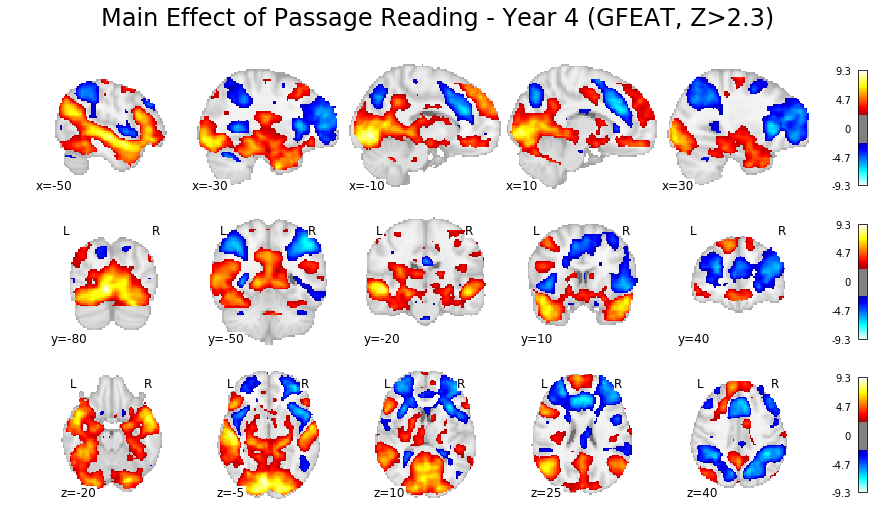
\includegraphics[width=5in]{Ch2_ActivationPassagesY4}
    \caption[Language comprehension spans many brain areas.]{A widespread set of brain areas are utilized during listening and reading comprehension, including auditory, default mode and attention areas.}
\label{fig:ch2_passages}
\end{figure}

Differences related to modality fell into three categories: sensory processing areas, including the insula, superior temporal gyrus, and secondary visual processing areas; and hetero-modal association areas, most notably the inferior frontal gyrus and angular gyrus; and somato-motor regions, including the premotor cortex and lateral geniculate nucleus of the thalamus (Figure 2). Areas related to listening were focused on primary auditory cortex and the dorsal attention network. Areas related to reading spanned a larger 

\begin{figure}[!b]
\centering
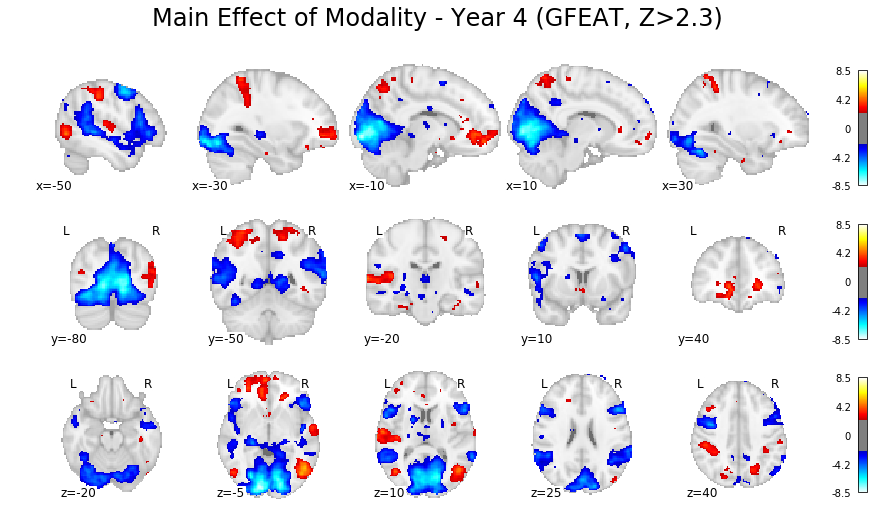
\includegraphics[width=5in]{Ch2_ActivationModalityY4}
    \caption[Modality differences center on primary sensory and integration areas.]{Modality differences center on primary sensory and integration areas.}
\label{fig:ch2_modality}
\end{figure}

Covariate analyses in Grade 3 revealed significant correlations between the linguistic principal component and comprehension-related brain activity in the posterior cingulate cortex, a key node of the default mode network (Figure 3). No relationships were found between the reading principal component for comprehension activity. No relationships were found between either principal component and modality differences.

Findings were highly conserved across years and within-subject. No significant age-related differences were found when treating the subjects cross-sectionally (Grade 3 Group vs. Grade 4 Group) or as paired t-test (n = 30). Intersection analyses revealed that a high percentage of voxels that exhibited significant main effects in Grade 3 were also significant in Grade 4 (___ percent for supra-modal effects, ___ percent for uni-modal effects).

\subsection{Classification}
When tested on the grade 4 data, the classifier was able to correctly identify 83 percent of the data, suggesting that the “supra-modal core” does indeed contain a pattern of information which is influenced by modality. Report other metrics….

\subsection{Connectivity}
Because minor changes to network-forming thresholds can influence these properties, all analyses were performed across a range of thresholds. Values reported here are using a threshold of Pearson’s r = 0.20. The trends reported here are robust across a range of thresholds (Supplemental Figure 1). 

Passages vs. Rest: Across the whole-brain network, reading increased the global efficiency (t = ___, p = ____) and ____ the clustering coefficient decreased (t = ___, p < 0.001).
Listening vs. Reading: Across the whole-brain network, reading increased the global efficiency compared to listening (t = -3.167, p = 0.0013). No global changes were found for the clustering coefficient. However, at the regional level, areas which were associated with high modality-specific effects in reading also exhibited decreased clustering coefficients (G3, p < 0.001; G4, p < 0.001) (Figure 5). This effect was seen predominantly in nodes that were, at rest, involved in the visual network, suggesting that during reading a large portion of the visual network becomes more externally connected to other areas. This may be the key driver of the overall increase in global efficiency.


\section{Discussion}